\chapter{Introduction and Background}
\label{litreview}

\section{Introduction}
\paragraph{}
The quest of achieving autonomous driving is not new, much research has been focused on this area since the early 1990s. Sign detection is part of that quest and so gets a fair amount of attention by the research community and industry alike. The applications range from experimental self-driving vehicles to common driver assistance hardware. The constant progress of computer vision techniques and the progress made on hardware constantly reshape the boundary of possibility to run real time detection on low end embedded hardware.

In this Chapter we will review the different methods explored by the research community to try to solve traffic sign detection problem. We will first focus on the pre-deep learning area algorithms, which will be noted as classical algorithms in this document, and try to exhibit the different methods they tried and how they already incorporated machine learning to improve their results. We will then focus on how deep learning changed image processing and introduce some state of the art object detection models. We also explore new possibilities offered by approaches like architecture search and the current focus on mobile devices.

\section{Traffic sign detection}
\paragraph{}
Traffic sign detection has a long history that started as soon as RGB digital camera became available. In 1993, \cite{janssen1993hybrid, besserer1993shape} were already trying to solve this problem. The approach proposed by \cite{janssen1993hybrid} is based on per color pixel classification to segment the potential sign on the image followed by a pictogram classifier, while the approach proposed by \cite{besserer1993shape} reposed on grayscale image to lower the computation requirement and used multi-scale grayscale segmentation to extract shapes and classify them.

Some autonomous prototypes were also developed in the year 1994 \cite{ulmer1994vita}. The vehicle presented in \cite{ulmer1994vita} needed an additional $1400W$ power supply to run the embedded equipment while the document states "the complexity of this [traffic sign] recognition task".

With the progress of computer vision and computational power of computers, more complex approachs have now been explored. \cite{de1997road} proposes a method based on color threshold and edge detection to perform this task and introduces a fully connected neural network to perform the classification. Another method of threshold using both HSV and YUV color space to better take into account the different illuminations was proposed in \cite{shadeed2003road}, while \cite{bahlmann2005system} proposed a new approach using Haar wavelet transform of the image and performing detection by extracting features of this transformation based on an Ada-boost trained classifier.

As more computational power became available, it became clear that computer vision algorithms needed machine learning to fine tune their algorithms, and as such data started to appear as a cornerstone of this task. In addition, the rapid development of the world wide web provided an easy way to share data across the scientific community, making the process of comparing results easier. Data set such as GTSDB \cite{gtsdb} quickly appeared to fill that gap, proposing a set of one thousand images from German roads, properly annotated, to the community. Other data set quickly followed such as \cite{mathias2013traffic} in Belgium or \cite{larssonSCIA2011} in Sweden.

\paragraph{}
The methods presented above manage to get good accuracy on detection with a relatively low computation budget by today's standards. However, the results often lack the repeatability needed for real word application and are specific to the setup of the authors.

\section{Deep learning}
\paragraph{}
Since the demonstration done with AlexNet \cite{alexnet} on the ImageNet \cite{deng2009imagenet}, deep learning have received much attention from the research community and the industry. This interest lead to major breakthroughs in computer vision tasks, starting from image classification and propagating to object detection, image segmentation or image captioning. This revolution in the computer vision field was lead by the use of powerful GPU allowing running complex models.
\subsection{Image Classification}
\paragraph{}
AlexNet \cite{alexnet} opened the gate to a large amount of innovation. Resnet \cite{szegedy2017inception} showed that residual connection allowed the gradient to propagate further in the network.

Other architecture such as MobileNet \cite{sandler2018mobilenetv2, howard2019mobilenetv3} were also developed to fit particular hardware platforms or tasks. Trying to be more optimized for mobile devices by using operation that are more efficient on a sequential CPU, and not on big parallel GPU as it is usually done.

\subsection{Object detection}
\paragraph{}
Object detection was part of the second wave of deep learning. In this case, this new approach also allowed to reach accuracy never reached before. The goal here is to have a system that provides boxes around a specific set of objects when given an image. This field is dominated by two approaches that now tends to get closer and closer.

The first approach to solve this problem was to first have a region proposal network that detects objects and a classifier giving the class of the object. This approach was successfully shown in RCNN \cite{girshick2014rich}, but the process was later shown to be inefficient and was streamlined into a single module in Fast-RCNN \cite{girshick2015fast} allowing a faster detection speed and a single stage training. This process was improved even more in Faster-RCNN \cite{ren2015faster}, which makes the detection even faster by using the same feature extraction layers for region proposal and object classification, cutting the computation time required, but was still not able to reach real time object detection even on big GPU.

The second approach is very similar to Faster-RCNN in that it needs only to run on the image once and use the same feature extraction for all the predictions, but instead of doing a two steps process, here the networks predict directly the bounding boxes shape and class on the same layer. Usually these prediction layers are then placed at different depths of the network to manage different sizes. This approach was first demonstrated on YOLO \cite{yolov3}, allowing running detection real time with only a small accuracy loss over Faster-RCNN. This process was generalized with SSD \cite{liu2016ssd} that follows the same idea but with small changes that make it easier to use with different backbone networks.

One common point of the object detection methods is that they have a tendency to predict multiple boxes for the same object. To remove that problem, a post processing step is often needed. Usually this post processing is done by a non max suppression algorithm. This algorithm takes as input a threshold value between $0$ and $1$, and compares the intersection over union of each predicted boxes pair, removing one of the boxes if this value is higher than the threshold and leaving only the box with the higher confidence level. This approach allows to remove most of the duplicate detection, even if it sometimes harm the results in case of superposing objects.

Object detection is now a problem that is considered to be nearly solved by the research community, as models like Yolo and Faster-RCNN manage to achieve above human performance. However, getting this kind of results require both a very large amount of data for training as well as a very powerful GPU to run it at a reasonable frame rate.


\subsection{Architecture search} \label{architectureSearch}
\paragraph{}
Architecture search is currently a very active area in the research community. It is also a problem that is still unsolved. This area of research start from the observation that the current network architectures used globally are designed by experts to solve their current problems. However, these networks are limited to specific problems and may not be optimal to solve other problem. The idea is then to train a computer to generate architecture that can be trained and achieve better or as good as human designed ones.

The most common approach to this problem is to train a network to design another network. This is usually done with a Recurrent Neural Network (RNN) trained using Reinforcement Learning (RL) to design an architecture \cite{zoph2016neural}.

Another approach is to rely on genetic algorithm to select the evolution of the network. This technique was demonstrated in \cite{real2019regularized} and showed impressive results on the ImageNet \cite{deng2009imagenet} image classification challenge. 

The last way that is currently investigated is to make the architecture differentiable so that you can train it at the same time as the weights during gradient decent. This method was successfully used in \cite{liu2018darts} and show interesting results in term of training time as well as quality.

The above approaches are usually combined with more classical exploration approaches like NetAdapt \cite{yang2018netadapt}, which tries to further improve the global architecture to a target device. 

However, those approaches still require a fair amount of time and computing power. In addition, this research area mainly focuses on image classification so far, and being a very active topic there is no reference implementation.

\subsection{Mobile device} \label{subsec:optMobileDevice}
\paragraph{}
Nowadays the problem of object detection is largely solved. It still requires a large amount of data which are not available in every field, but given enough data you can detect objects in real time with while being more accurate than humans. However, this approach is still very heavy in computations and require large computer and GPU to run effectively. This causes trouble for many applications where you would like to process the data while collecting them, either because you need to interact with your environment or because you cannot manage the data generated by recording everything. In addition, most of the time you cannot afford to bring a powerful computer with GPU to collect your data and prefer to use more broadly available devices.

The first step in improving performance is to scale the network down, this can be done in multiple ways, as discussed in Section \ref{architectureSearch}. To improve further you have to go to hardware specific optimization. In this area, weight quantification is the most used technique. This approach consists of changing the commonly used 32 bits floating-point values to 8 bits integer values. A method leveraging SSE instruction set on an Intel CPU can provide large speed up to the run time when combined to conversion from floating-point to integer value was presented in \cite{vanhoucke2011improving}. \cite{jacob2017quantization} and \cite{gysel2016hardwareoriented} show that a similar approach can be used for mobile devices and have shown to have a large impact on prediction speed of the optimized networks.

However, optimizing the network further is not always possible. To make devices smarter, manufacturers now bundle more and more computational power in their devices. Smartphones are a good demonstrator of this trend, with newer models getting much larger and accessible parallel computation unit, sometimes even proposing additional chip to run neural networks. Following this trend Google is developing a smaller version of their TPU for mobile device under the name Coral. A similar trend is going on Internet Of Things (IoT) devices. Completing computations on site is a key factor to save space and bandwidth. Coral devices are not the only one the to target this; Nvidia released many different development board with large integrated GPU with a strong incentive on self driving cars.

\subsection{Training}
\paragraph{}
One of the biggest challenges of machine learning is overfitting. Artificial neural networks are very sensitive to this because of the high number of parameters they use. Because of that they are also very difficult to train on a reasonable time scale. These problems are well known and were subject of lot of research, leading in large improvements on that field. We are going to quickly cover some of the improvements that are used in this work.

The original inspiration for artificial neural network are the real neural networks we find in animals brains. Much of early design choices were made following this idea. A good example of that is the activation function. Activation function need to be non-linear to add expressivity to the network and prevent it from being collapsible into one linear function. Originally, $sigmoid$ function was used as they provided a good equivalent to animal brains, this function was later ruled out by $tanh$ that provided easier training by centering the output values around zero. However, this function is computationally intensive and was later replaced by ReLu, a function defined as $ReLu(x) := max(0,x)$. This function was proven to allow good training while making it easier to compute. Cropping this activation function upward has also been proven to be more effective on mobile devices \cite{sandler2018mobilenetv2, howard2019mobilenetv3}, leading to the adoption of the ReLu6 function, defined as $ReLu6 := min(6,ReLu(x))$. The research on activation function is still ongoing, the sift activation function used in \cite{howard2019mobilenetv3} has allowed to improve the results, but at a higher computational cost. In this study we chose to use the ReLu6 activation function for its efficiency.

It quickly became apparent that the distribution of the activation in the hidden layer was slowing down the training. Instead of expecting the gradient decent to fix that during training, one approach was shown to be very successful, batch normalization \cite{ioffe2015batch}. Batch normalization learns during the training to do an approximate normalization over each training batch and applies it during prediction time, making the following layers more effective.

Batch normalization has a tendency to reduce overfitting, but is far from solving this issue. On image based network, like in this work, it is easy to tweak the images slightly to add more diverse cases to the training and prevent the network from overfitting the training data. These modification are usually color shift, brightness change, or linear transformation such as rotation, translation and zoom. A more generic approach to prevent this problem is Dropout \cite{srivastava2014dropout}. This approach proposes to randomly disable connection in a neural network during the training, forcing the network to build some redundancy and preventing it from relying on only one feature. This approach has proven to be very effective in a large spectrum of cases across all fields where neural networks are used. However, the final results will always depend on the quality and quantity of real world data available.

This is only a quick review of the most used ways to improve neural network training time and accuracy, focusing on the methods we are going to use in this study.

\section{Metrics}
\subsection{Introduction}
\paragraph{}
In this work we are going to use different metrics to evaluate our results. The reader who is already familiar with the concept of IoU or mAP may decide to skip this section.

\subsection{Intersection over Union}
\paragraph{}
Intersection over Union or IoU, is the most used way to check if two objects are correctly overlapping or not. The name of this metric is self explanatory: the value of this metric is the value of the division of the area of the intersection over the area of the union, as you can see illustrated on Figure \ref{fig:iou}.

\begin{figure}
    \centering
    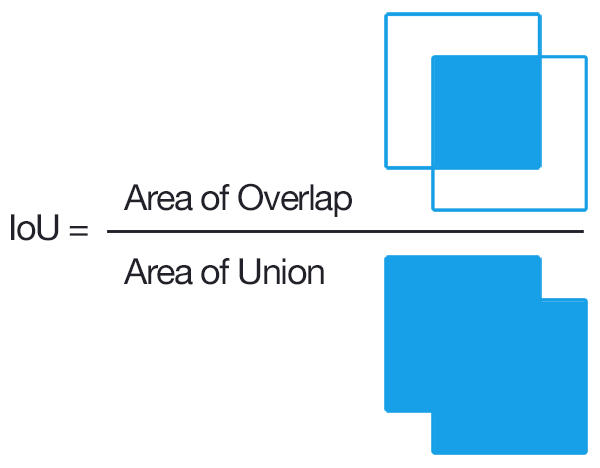
\includegraphics[width=0.3\linewidth]{figures/Intersection_over_Union_-_visual_equation.png}
    \caption{Illustration of intersection over union equation from \cite{wiki:iou}}
    \label{fig:iou}
\end{figure}{}

The value of this metric is equal to one if and only if the to area are exactly overlapping. The value decrease to zero as the overlapping become less important, taking into account the fact that one of the object may be inside the other. This makes it a great metric to compare a predicted box with a ground truth box.

\subsection{True positive, false positive and false negative}
\paragraph{}
In a object detection context, True Positive, False Positive and False Negative, often written as TP, FP and FN, are values that, in a nutshell, represent respectively the count of detection matching the ground truth, not matching the ground truth and ground truth not matched with any detection. 

First we need to define what is a match between detection and ground truth. This is usually defined by using the IoU between the two boxes, creating a match if the IoU value is above a given threshold. In this work as it is generally the case in the literature, unless explicitly stated otherwise, the threshold we use is $0.5$. So a detection match a ground truth if the IoU between them is higher than $50\%$.

With that definition set, we can come back to the previous statement. If a detection is matched with a ground truth, this detection is counted as a TP. After matching, all the remaining unmatched detection are FP and the unmatched ground truth are FN.

For the sake of simplicity we skipped here the case of multiple detection matching the same ground truth. In this case the higher IoU match is kept, so the ground truth is only matched once.

\subsection{Precision and Recall}
\paragraph{}
Using the TP, FP and FN values defined previously we can build more meaningful metrics, such as precision and recall. As illustrated by Figure \ref{fig:precisionrecall}, precision and recall answers two different questions. The first answers the question of how many of detected objects are relevant, putting the incentive on the FP as a maximum precision can only be reach if there is no FP, but without paying attention to FN. On the other hand, recall tries to answer the question of how many of the truth object were detected, but without considering FP.

\begin{figure}
    \centering
    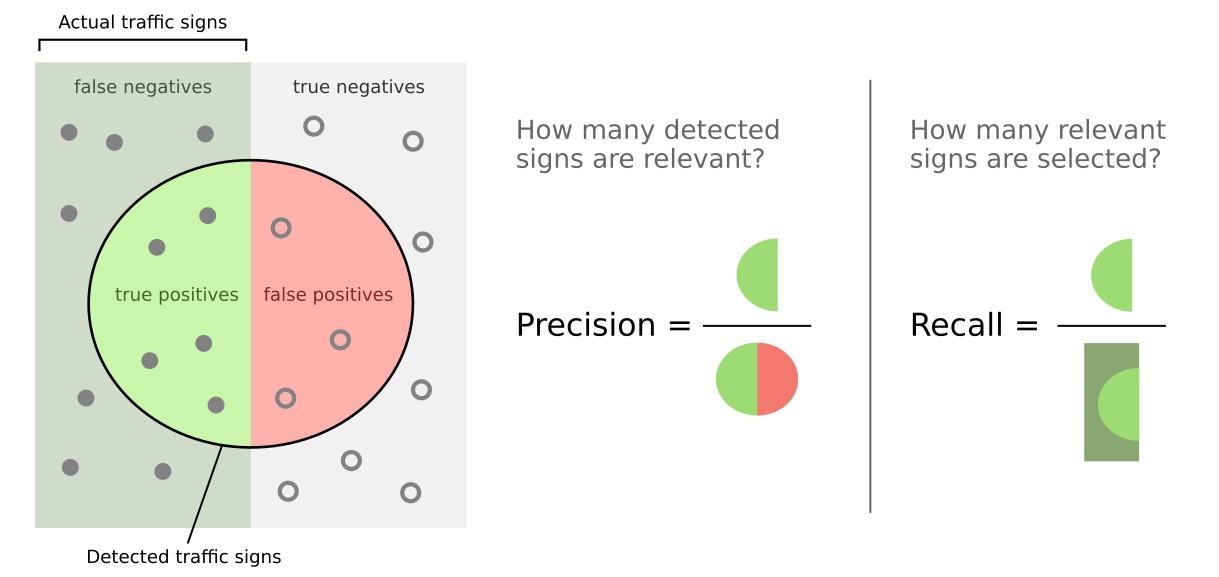
\includegraphics[width=0.8\linewidth]{figures/precisionrecall.png}
    \caption{Illustration of the precision and recall in the traffic sign detection context. Modified from \cite{wiki:precisionrecall}}
    \label{fig:precisionrecall}
\end{figure}{}

To get a perfect recall, one can detect everything, and so be sure not to miss any detection, but that will produce a lot of FP, decreasing the precision to very low values. Following the same idea, to get a perfect precision, one can detect only the one object it is most confident in, but that will result in very high FN and so low recall. This quick analysis shows the importance of correlating these two metrics to get meaningful results.

\subsection{Mean Average Precision}
\paragraph{}
Mean average precision, usually written as mAP, is the most used metric in object detection problem. This metric is more difficult to describe than the previous one, and is sometimes the subject of an entire paper by itself, for more information we advise you to consult \cite{wiki:metrics}.

As a quick description, mAP is the mean of the average precision (AP), which is computed for every classes. Average precision is the area under the curve of the recall vs precision graph where each point correspond to a confidence level. In other word, the AP is one if for any confidence level the recall and precision are equal to one.

Usual mAP is defined for a threshold of IoU with ground truth of $50\%$. But this research as well as lot of recent papers will use the notation $mAP@th$, where $th$ is the IoU threshold used to get the value of this metric. For example $mAP@50$ is the $mAP$ computed for detection matched with ground truth if they have an IoU higher than $50\%$.

\section{Conclusion}
\paragraph{}
Traffic sign detection and more broadly object detection have received a lot of attention from the research community over a large period of time. The rapid development of deep learning allowed great breakthroughs in this area, but the problem of getting similar level of accuracy real time on mobile devices is still largely unsolved. Improving the performance of the device is a solution to this problem, but optimization and fine-tuning is the key to achieve good results.

